\documentclass{article}
\usepackage{enumitem}
\usepackage{graphicx} % Package to handle images

% Title and Author
\title{19CSE302 - Design Analysis Of Algorithms \\ Lab Evaluation 1}
\author{Praneeth V - CB.EN.U4CSE22244 \\ Sai Krishna - CB.EN.U4CSE22246}

\begin{document}

\maketitle

\section*{Lab Evaluation Questions}

\begin{enumerate}
    \item Analysis of Sorting algorithms
    \begin{enumerate}[label*=\arabic*.]
        \item In-Place Quick Sort (with last element as the pivot)

        Quick sort applies the Divide-And-Conquer strategy to sort a subarray A[p..n]:


        \textbf{Divide} : The array is rearranged into two subarrays such that A[p .. q-1 ] is less than that of A[q] and the other subarray A[q+1 .. n] 
        greater than A[q]. Here A[q] is the pivot element.

        \textbf{Conquer} : We sort the subarrays A[p .. q-1] and A[q+1 .. n]

        \textbf{Combine}: Now, we combine the sorted arrays together. 

        The time complexity of the In-Place Quick Sort depends on whether the partitioning is balanced or not, and depends on which elements are used for partitioning. 

        If the partitioning is balanced: It's the best case where the algorithm runs as fast as merge sort. Since the partitioning is balanced, we get two even halves where one is of the size \( \lfloor n/2 \rfloor \) and the other one of the size \( \lfloor n/2 \rfloor - 1 \). So the recurrence relation for this becomes: \( T(n) = 2 T(n/2) + \Theta(n) \) and by Master's Theorem, it becomes \( T(n) = \Theta(n \log n) \). 

        If the partitioning is unbalanced: Its the worst case where we have one subarray with size of \( n-1 \) and the other subarray with the size of 0. The time complexity of the partitioning costs \( \Theta(n) \) time and the recurrence relation for this case becomes:
        \( T(n) = T(n - 1) + \Theta(n) \) and making the overall time complexity \( T(n) = \Theta(n^2) \) and this case mostly happens when the array is already sorted. 

        If the partitioning is based on proportionality: Its the average case where the partitioning is done based on some proportions where the partitioning is like x-to-\(10-x\), then in this case the recurrence relation becomes like: \( T(n) = T(x \cdot n/10) + T(n/10) + c \cdot n \) in which just reaching the depth of the recursion tree for partition takes \( \log_{10/x} n \) which is \( \Theta(\log n) \) and the cost at each level is \( n \) making the time complexity: \( T(n) = O(n \log n) \)

        The Space complexity for In-Place Quicksort is \( O(\log n) \) for best and average case partitioning where \( logn \) represents the size of the recursion tree and in the worst case partitioning the space complexity becomes \( O (n) \) as the recursion tree becomes skewed leading to the size of the tree to be equal to the number of elements in an array. 

        % Code Section 1.1.1
        \begin{verbatim}
        Test Case 1: For size 100:
        \end{verbatim}

        % Image Section 1.1.1
        \begin{figure}[h]
            \centering
            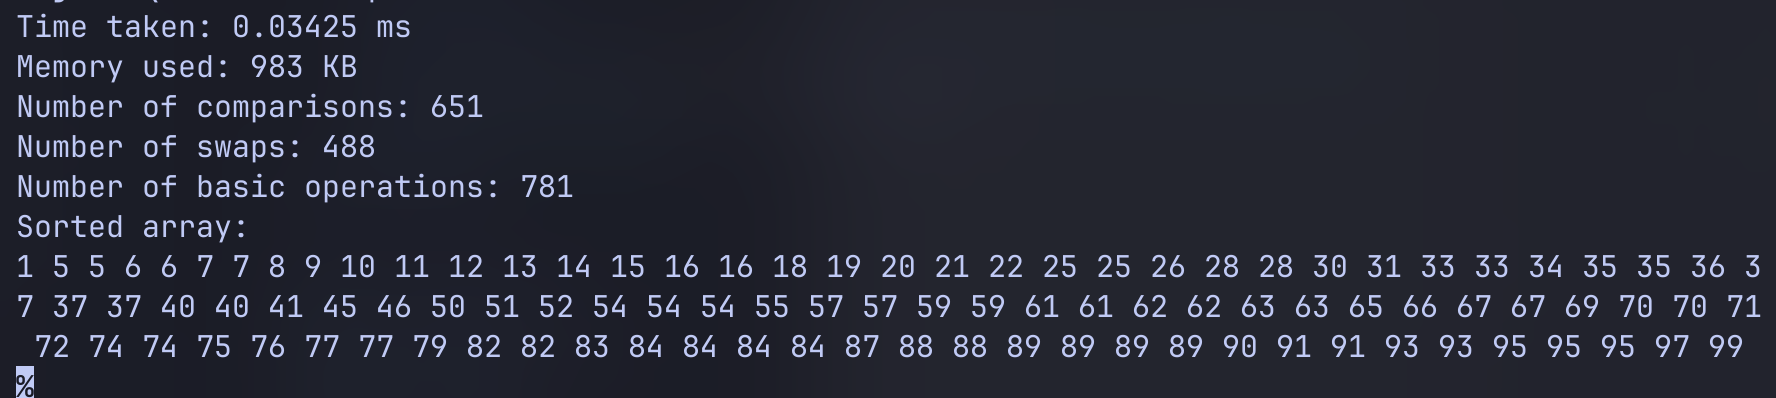
\includegraphics[width=0.8\textwidth]{./quicksort-tc-1.png}
            \label{fig:image1}
        \end{figure}

        % Code Section 1.1.2
        \begin{verbatim}
        Test case 2: For size 300
        \end{verbatim}

        % Image Section 1.1.2
        \begin{figure}[h]
            \centering
            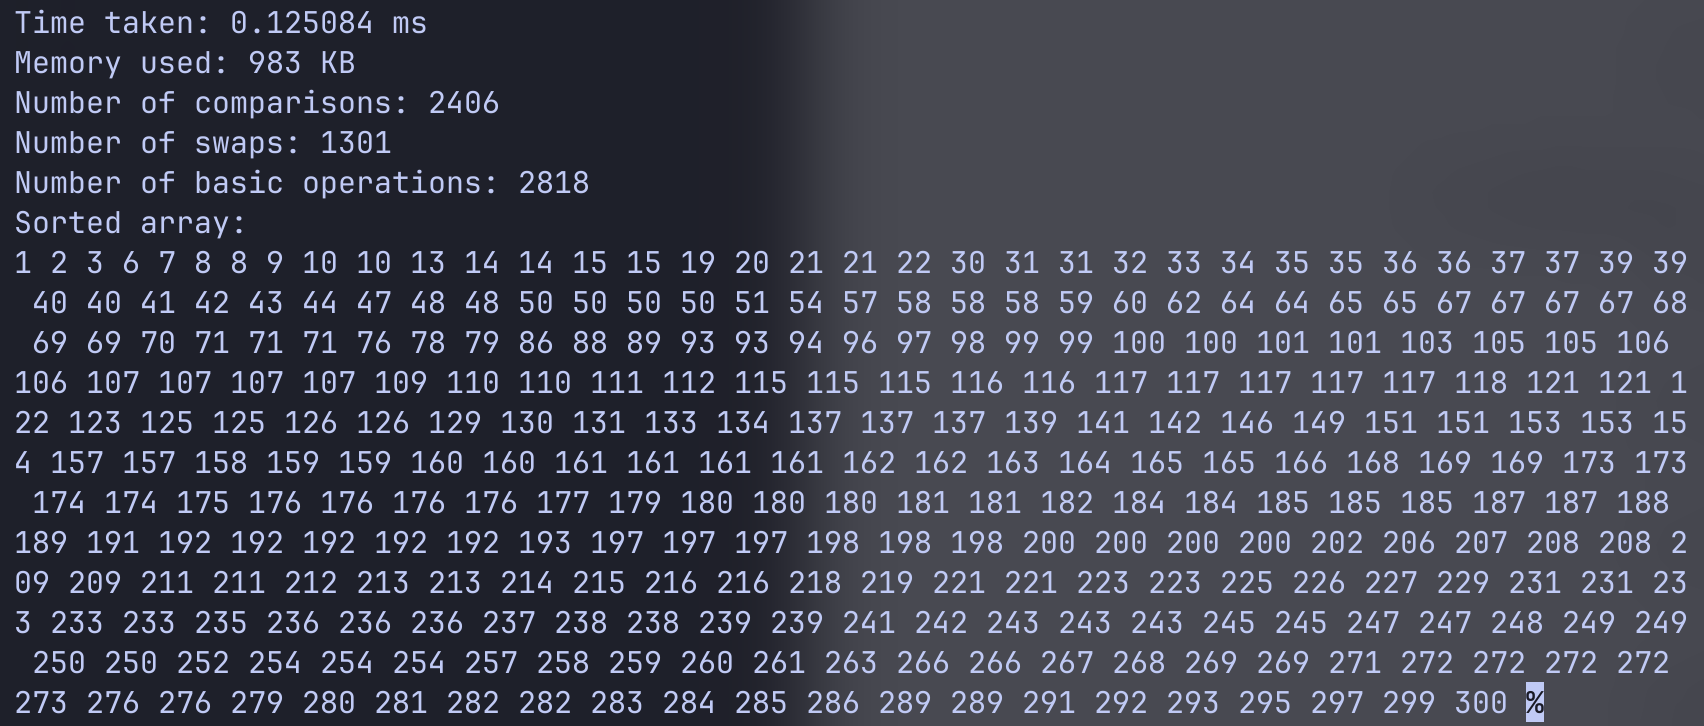
\includegraphics[width=0.8\textwidth]{./quicksort-tc-2.png}
            \label{fig:image2}
        \end{figure}

        % Code Section 1.1.3
        \begin{verbatim}
        Test case 3: For size 500
        \end{verbatim}

        % Image Section 1.1.3
        \begin{figure}[h]
            \centering
            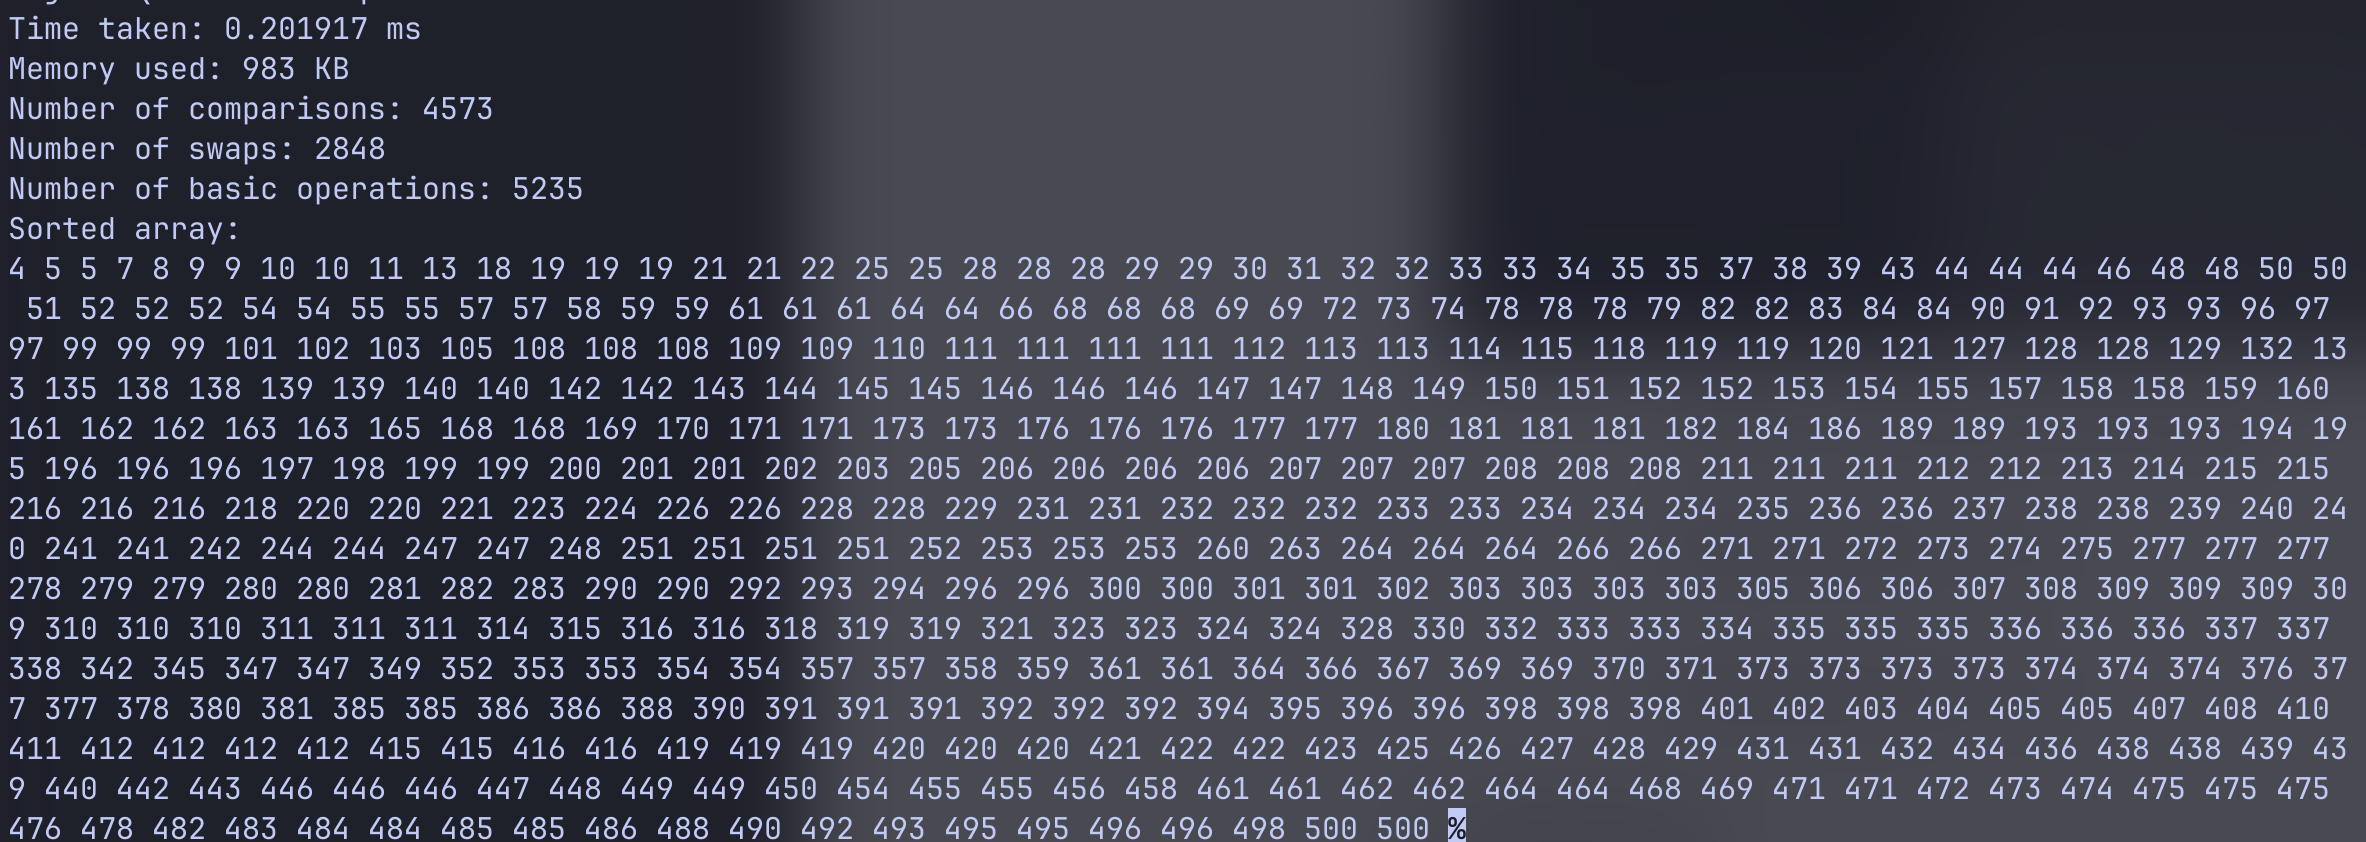
\includegraphics[width=0.8\textwidth]{./quicksort-tc-3.png}
            \label{fig:image3}
        \end{figure}

        % Code Section 1.1.4
        \begin{verbatim}
        Test case 4: For size 1000
        \end{verbatim}

        % Image Section 1.1.4
        \begin{figure}[h]
            \centering
            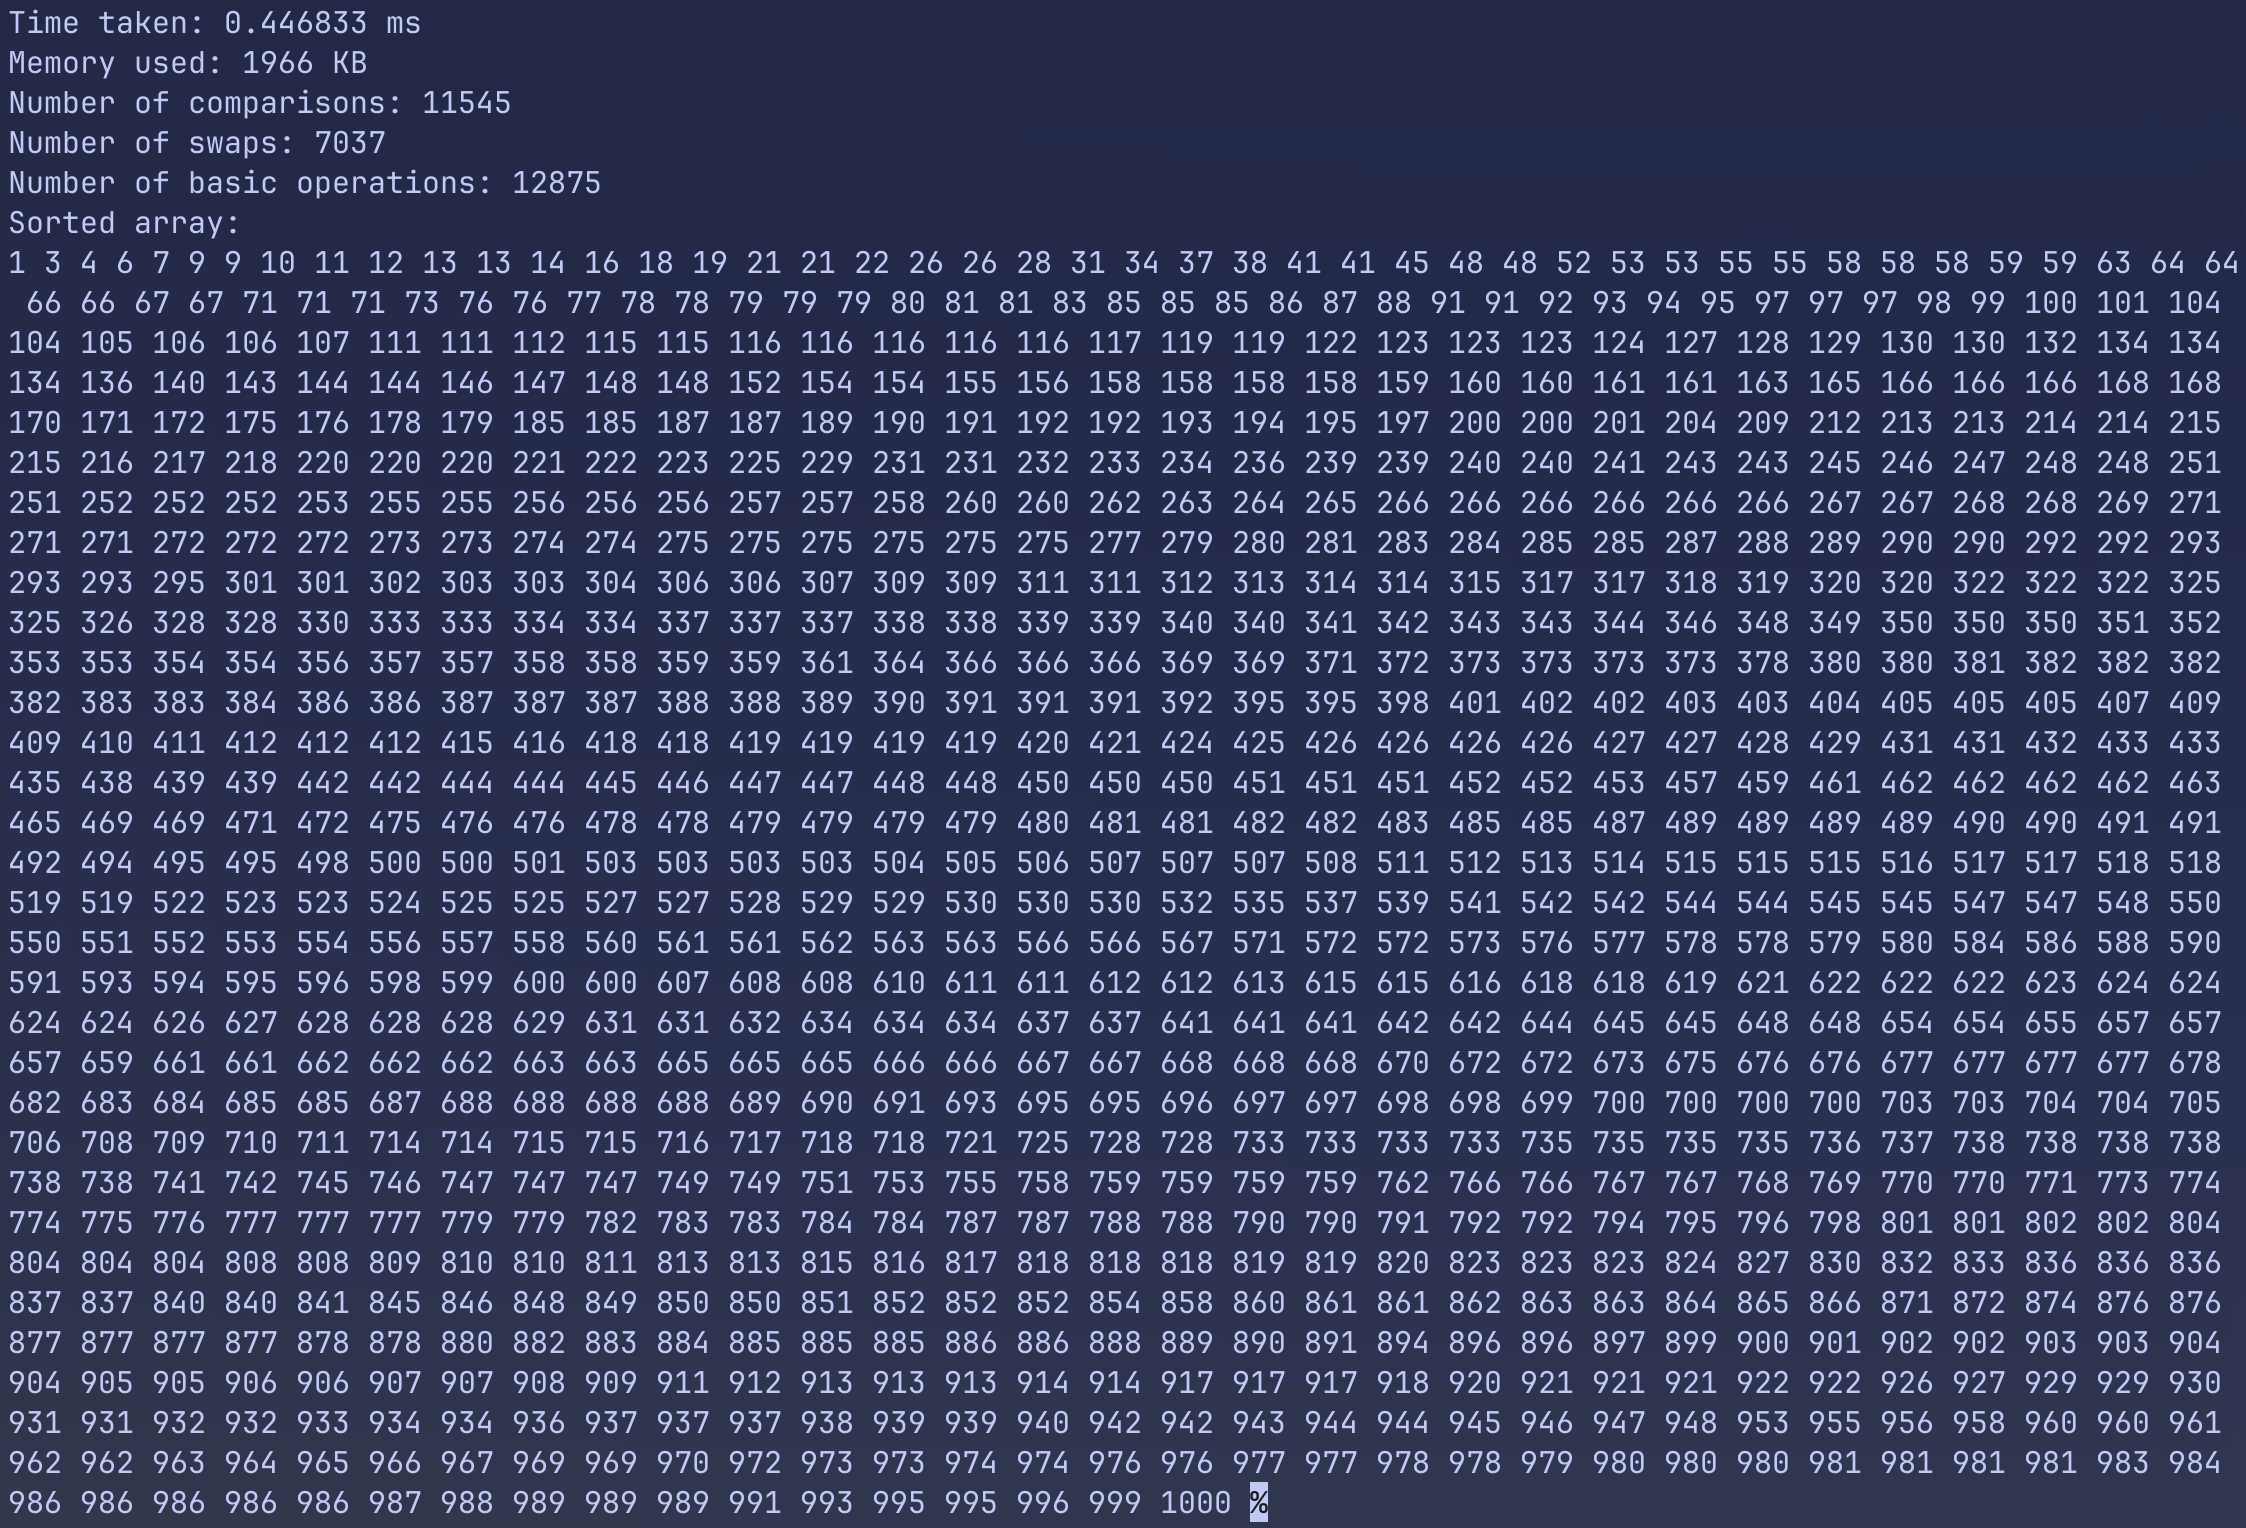
\includegraphics[width=0.8\textwidth]{./quicksort-tc-4.png}
            \label{fig:image4}
        \end{figure}

        \item Three-way merge sort

          Merge sort applies the Divide-And-Conquer strategy to sort an array A[p .. n]. 

        % Code Section 1.2.1
        \begin{verbatim}
        % Code Section 1.2.1
        \end{verbatim}

        % Image Section 1.2.1
        \begin{figure}[h]
            \centering
            \includegraphics[width=0.8\textwidth]{path/to/image5.png}
            \caption{Description of the image}
            \label{fig:image5}
        \end{figure}

        % Code Section 1.2.2
        \begin{verbatim}
        % Code Section 1.2.2
        \end{verbatim}

        % Image Section 1.2.2
        \begin{figure}[h]
            \centering
            \includegraphics[width=0.8\textwidth]{path/to/image6.png}
            \caption{Description of the image}
            \label{fig:image6}
        \end{figure}

        % Code Section 1.2.3
        \begin{verbatim}
        % Code Section 1.2.3
        \end{verbatim}

        % Image Section 1.2.3
        \begin{figure}[h]
            \centering
            \includegraphics[width=0.8\textwidth]{path/to/image7.png}
            \caption{Description of the image}
            \label{fig:image7}
        \end{figure}

        % Code Section 1.2.4
        \begin{verbatim}
        % Code Section 1.2.4
        \end{verbatim}

        % Image Section 1.2.4
        \begin{figure}[h]
            \centering
            \includegraphics[width=0.8\textwidth]{path/to/image8.png}
            \caption{Description of the image}
            \label{fig:image8}
        \end{figure}

        % Continue with similar structure for other code sections
    \end{enumerate}

    % Repeat the above structure for other sections and questions
    % Make sure to replace "path/to/imageX.png" with the actual path to your image files
    % and provide appropriate captions and labels.
\end{enumerate}

\end{document}

